\documentclass[10pt,a4paper,twocolumn]{article}

\usepackage[english]{babel}
\usepackage{float}
\usepackage{lipsum}

\input{pisika.dat}

%  Editorial staff will uncomment the next line
% \input{staff.hed}
\usepackage{tikz}
\usetikzlibrary{positioning, calc}

%% acronyms and glossary
\usepackage[
    single=true,
    sort=true,
    only-used=true
]{acro}
\DeclareAcronym{UWB}{
    short = UWB,
    long = Ultra-Wideband
}

\DeclareAcronym{TWR}{
    short = TWR,
    long = Two-Way Ranging
}

\DeclareAcronym{EKF}{
    short = EKF,
    long = Extended Kalman Filter
}

\DeclareAcronym{NLOS}{
    short = NLOS,
    long = Non-Line-Of-Sight
}

\DeclareAcronym{RTOS}{
    short = RTOS,
    long = Real-Time Operating System
}

\DeclareAcronym{TOF}{
    short = TOF,
    long = time-of-flight
}


%% Pictures
\renewcommand{\figurename}{Figure}

\begin{document}

%--------------------------------------------------------------------------
%  fill in the paper's title, author(s), and corresponding institutions
%--------------------------------------------------------------------------
\providecommand{\ShortAuthorList}[0]{S. Krebs, T. Herter} % use "A.~M.~Surname \textit{et al}." for more than three authors.
\title{Ultra-Wideband (UWB) Positioning System Based on ESP32 and DWM3000 Modules}
\author[1]{Sebastian Krebs}
\author[1]{Tom Herter}
\affil[1]{HTWG Konstanz,\linebreak  Faculty of Electronics und Informationtechnologies,\linebreak Germany}
%\affil[2]{Other Institute, XX University}

\date{\dateline{\today}}

\maketitle
\vspace*{-1.3cm}
%\thispagestyle{titlestyle}

\section*{}
%---------------------------------------------------------------------------
%               Include abstract and keywords here
%---------------------------------------------------------------------------
\textbf{\textit{Abstract}} - \textbf{
  In this paper, we introduce an innovative \ac{UWB} positioning system
  that leverages six identical custom-designed boards,
  each featuring an ESP32 microcontroller and integrated with DWM3000
  modules from Quorvo.}

  \textbf{This system is capable of achieving precise localization through \ac{TWR}
  measurements between one designated ''Tag'' board and five other ''Anchor'' boards.
  The collected distance measurements are processed by an \ac{EKF} running locally
  on the Tag board, enabling it to determine its own position with high accuracy,
  relying on the fixed positions of the Anchor boards.}

  \textbf{This paper presents a comprehensive overview of the system's architecture,
  the key components, and the remarkable capabilities it offers for accurate
  indoor positioning and tracking applications.}

\vspace*{.28cm}
\keywords{\textbf{RTLS, UWB, TOF, ESP32, DWM3000, Positioning, Tracking}}

%---------------------------------------------------------------------------
%               the main text of your paper begins here
%---------------------------------------------------------------------------

\section{Introduction}\label{section:intro}
Indoor positioning and tracking have become increasingly important in various areas,
such as logistics, healthcare, industrial automation and smart infrastructures.
Conventional positioning systems often face challenges in terms of accuracy, scalability and robustness.
To solve these problems, we present a \ac{UWB} positioning system that utilizes
hardware and advanced algorithms,
The result is an exceptional level of accuracy and reliability.

Our \ac{UWB} system consists of six identical boards,
all based on the ESP32 microcontroller, a versatile and powerful platform that is 
known for its capabilities in wireless communication and processing.
These boards are equipped with DWM3000 modules from Quorvo,
which are known for their powerful UWB capabilities.

One of these boards is referred to as a ''tag'',
It is responsible for initiating measurements with the other five "anchor" boards.
The innovative aspect of our system lies in its ability to perform accurate localization
without dependence on external infrastructure or centralized processing.

The heart of our \ac{UWB} system is the \ac{EKF} implemented locally on the tag board.
This \ac{EKF} takes the distance measurements obtained by \ac{TWR} with the Anchor Boards and calculates,
and, based on their known fixed positions, calculates the real-time position of the tag board
with remarkable precision.
This decentralized approach not only ensures fast and reliable positioning, but also scalability and is therefore
scalability and is therefore suitable for various applications where real-time position data is critical.

In this paper, we will look at the details of our \ac{UWB} system.
We will explain the hardware structure and firmware architecture.

\section{Measurement Priciple}\label{Section:principle}
\acf{TWR} is our foundational technique for obtaining precise distance
measurements within the UWB positioning system.
It relies on the time it takes for signals to travel from a Tag board to Anchor boards
and back again.
This temporal measurement, in compliance with the IEEE 802.15.4a/4z standards,
offers the basis for distance estimation.

The following Figure \ref{fig:twr} shows how a
\ac{TWR} Handschake is done.
The Tag Firmware calculates the \acf{TOF} aswell
as the distance between both devices by comparing the
timestamps of sending and reception.

\begin{figure}[H]
  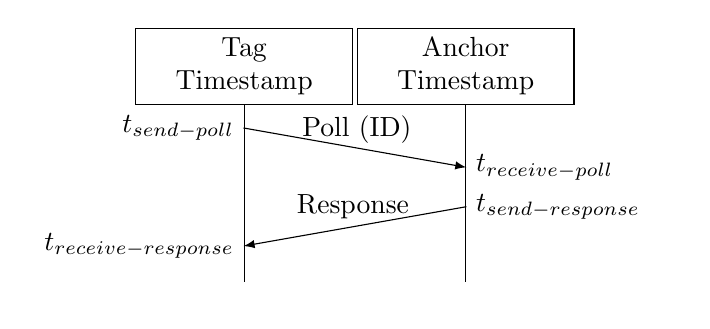
\begin{tikzpicture}[
    node distance=1.5cm,
    block/.style={
      align=center, draw,minimum width=2.75cm, minimum height=.5cm
    },
    ghost/.style={
      align=center,minimum width=0cm, minimum height=0cm
    },
    label/.style={
      minimum width=2cm, minimum height=0cm, text width=2.5cm
    },
    >=latex,
  ]
    % textfields
    \node [block] (tag_timestamp) {Tag\\Timestamp};
    \node [block, right=.05cm of tag_timestamp] (anchor_timestamp) {Anchor\\Timestamp};

    % Endpoints
    \node [ghost, below=2.25cm of tag_timestamp] (tag_endpoint) {};
    \node [ghost, below=2.25cm of anchor_timestamp] (anchor_endpoint) {};

    % Timelines
    \draw [-] (tag_timestamp) -- (tag_endpoint);
    \draw [-] (anchor_timestamp) -- (anchor_endpoint);

    % Labels Tag-line
    \node [label, align=right, anchor=east, below=.5cm of tag_timestamp.west] (t_send_poll) {$t_{send-poll}$};
    \node [label, align=right, anchor=east, below=2cm of tag_timestamp.west] (t_receive_response) {$t_{receive-response}$};
    
    % Labels Anchor-line
    \node [label, align=left, anchor=west, below=1cm of anchor_timestamp.east] (t_receive_poll) {$t_{receive-poll}$};
    \node [label, align=left, anchor=west, below=1.5cm of anchor_timestamp.east] (t_send_response) {$t_{send-response}$};

    %Dotted lines
    \draw [->] (t_send_poll.east) -- (t_receive_poll.west);
    \draw [->] (t_send_response.west) -- (t_receive_response.east);
    \node [ghost, below=.5cm of anchor_timestamp.west] (poll_label) {Poll (ID)};
    \node [ghost, below=1.5cm of tag_timestamp.east] (response_label) {Response};

  \end{tikzpicture}
  \caption{Timingdiagram of \acf{TWR}}
  \label{fig:twr}
\end{figure}

For detailed technical specifications and methods,
we refer interested readers to the Documentation of
the IEEE 802.15.4a/4z standards \cite{IEEE802154a} \cite{IEEE802154z},
which provides comprehensive guidelines for the
complex orchestration of \ac{UWB} signals and the calculation of \ac{TOF}.
These standards ensure the rigor and accuracy of our distance measurements,
They form the cornerstone of our \ac{UWB}-based positioning and tracking capabilities.

\section{System Architecture}\label{section:system_arch}
In our scenario, five Anchors are strategically distributed throughout the room,
positioned at a height of 4m on the ceiling to minimize the likelihood of 
\ac{NLOS} conditions.
These five Anchors do not possess information specific to their usage.

Customized settings, such as Anchor positions,
can be transmitted to the Tag within our designed system through a \ac{BLE} interface.
The Tag leverages these provided Anchor positions,
in conjunction with distance measurements,
to determine its own position accurately.

The following diagram illustrates the interactions between the individual components.
It is clear that when selecting the anchor positions,
should be evenly distributed along all three axes.
In addition, an overhead perspective helps to reduce measurement inaccuracies.

\begin{figure}[H]
  \centering
  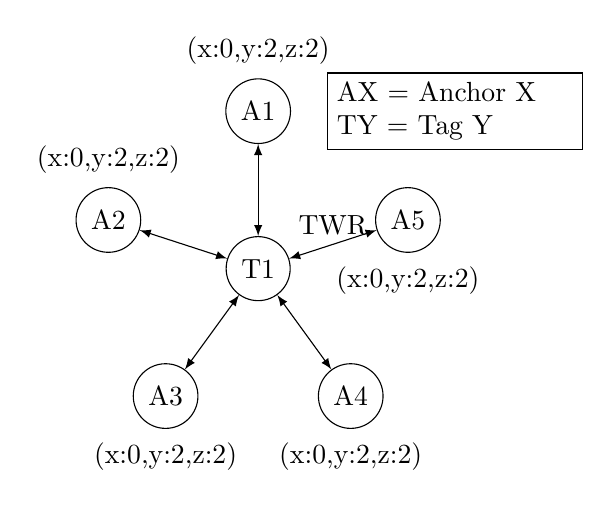
\begin{tikzpicture}[
    node distance=1.5cm,
    device/.style={
      align=center, circle, draw, minimum width=.25cm, minimum height=.5cm
    },
    ghost/.style={
      align=center,minimum width=0cm, minimum height=0cm
    },
    label/.style={
      draw, minimum width=2cm, minimum height=0cm, text width=3cm
    },
    >=latex,
  ]
    % Responders with coords
    \node [device] (device2) at (90:2cm) {A1};
    \node [ghost, above=.05cm of device2.north] (dev2) {(x:0,y:2,z:2)};
    \node [device] (device3) at (162:2cm) {A2};
    \node [ghost, above=.05cm of device3.north] (dev3) {(x:0,y:2,z:2)};
    \node [device] (device4) at (234:2cm) {A3};
    \node [ghost, below=.05cm of device4.south] (dev4) {(x:0,y:2,z:2)};
    \node [device] (device5) at (306:2cm) {A4};
    \node [ghost, below=.05cm of device5.south] (dev5) {(x:0,y:2,z:2)};
    \node [device] (device6) at (18:2cm) {A5};
    \node [ghost, below=.05cm of device6.south] (dev6) {(x:0,y:2,z:2)};

    %Initiator
    \node [device] (device1) at (0,0) {T1};

    % TWRs
    \draw [<->] (device1) -- (device2); 
    \draw [<->] (device1) -- (device3); 
    \draw [<->] (device1) -- (device4); 
    \draw [<->] (device1) -- (device5); 
    \draw [<->] (device1) -- node[midway, above, align=left] {TWR} (device6);

    %legend
    \node [label] (legend) at (2.5,2) {AX = Anchor X \\TY = Tag Y};

  \end{tikzpicture}
  \caption{Systemarchitecture for Positioning}
  \label{fig:systemarch}
\end{figure}

The round-trip time of the system is the product of the number of anchors and the ranging time.
The time for a distance measurement could be reduced to 50ms, which leads to a general position frequency of 250ms with 5 anchors.
This low ranging time of 50ms was achieved by implementing the firmware of the anchors interrupt-based in a multicore controller.

This strategic approach to Anchor placement not only optimizes
our positioning system's performance but also reduces the potential
for measurement errors.

\section{Hardware Design}\label{section:hardware}
The hardware design of our system draws inspiration from pre-existing DWM3000 Evaluation
boards.
However, our proprietary board development enables specialized component selection
tailored to their intended use cases.
User-friendliness was a paramount consideration during the design process,
resulting in the integration of multiple user buttons and LEDs.
Additionally, the PCB incorporates a convenient LiPo battery charging capability
via USB-C.

Notably, our PCB design ensures a consistent layout across all boards,
regardless of their specific application.
Below the antennas of both the DWM3000 and ESP32,
the ground plate has been selectively omitted to enhance antenna radiation
characteristics and enable more precise measurements.
This meticulous hardware design approach not only optimizes
performance but also prioritizes user convenience. 

\section{Firmware Architecture}\label{section:firmware}
To meet the demanding timing requirements essential for \ac{TOF}
measurements and enhance network round-trip times,
our firmware is implemented based on a \ac{RTOS}.
FreeRTOS \cite{FreeRTOS_2023}, in particular,
offers the capability to create multiple tasks that collaborate coherently
and can be executed simultaneously on each of the two cores of the ESP32 microcontroller.

The documentation of the source code is continuously made available online with the help of Doxygen and Github pages.
The implementation can therefore be viewed publicly\cite{doxygen-doku}.

In the regular tracking mode,
all devices within the system execute the TOF task, ensuring synchronized data acquisition.
When a device is configured as a Tag,
it additionally undertakes the execution of the \ac{EKF} task.
The \ac{EKF} task processes the distance measurements generated by the TOF task,
culminating in a precise positional estimation.

\subsection{TOF-Task}\label{section:firmware-tof}
The \ac{TOF} task in our system is based on the example code
provided by Quorvo for \acf{TWR} measurements.
However, we have refined the functionality by structuring it in a class-based framework.
The commonalities between the Initiator and Responder roles have been
encapsulated in a common superclass.
This design decision allows us to maintain a lean and clear software structure,
reduce redundancy and simplify maintenance.

In practice, the tag, which acts as the \ac{TWR} initiator,
iterates through a list of anchors, each of which serves as a \ac{TWR} responder.
The tag orchestrates distance measurements with each anchor,
The result is a comprehensive data set that serves as the basis for precise
precise localization indoors.

\subsection{EKF-Task}\label{section:firmware-ekf}
The \ac{EKF} employed in our system leverages two distinct mathematical models
to achieve precise position estimation.
For readers interested in delving deeper into the theoretical foundations of the
Kalman Filter, we recommend consulting the work of Li Qiang et al. in
"Kalman Filter and Its Application"~\cite{Kalman}.
The EKF  on the Tag utilizes a prediction model based on the constant velocity model assumption.
It posits that the tracked object moves with a consistent velocity along its recent
trajectory.
This model serves as a fundamental tool for forecasting the future position of the tag.

The measurement model is encapsulated in Equation~\ref{eq:measurementmatrix},
enabling the transformation of measured distances into accurate position estimations.
The measurement model finds its expression in the measurement matrix $H$,
which effectively links the measured distances to the position estimation:
\begin{equation}
  \begin{aligned}
    \Delta x_i &= x_i - x \\
    \Delta y_i &= y_i - y \\
    \Delta z_i &= z_i - z \\
    dist_i &= \sqrt{{\Delta x_i^2 + \Delta y_i^2 + \Delta z_i^2}} \\
    H &= \begin{bmatrix}
    -\frac{{\Delta x_1}}{{dist_1}} & -\frac{{\Delta y_1}}{{dist_1}} & -\frac{{\Delta z_1}}{{dist_1}} \\
    -\frac{{\Delta x_2}}{{dist_2}} & -\frac{{\Delta y_2}}{{dist_2}} & -\frac{{\Delta z_2}}{{dist_2}} \\
    \vdots & \vdots & \vdots \\
    -\frac{{\Delta x_{\text{max}}}}{{dist_{\text{max}}}} & -\frac{{\Delta y_{\text{max}}}}{{dist_{\text{max}}}} & -\frac{{\Delta z_{\text{max}}}}{{dist_{\text{max}}}}
    \end{bmatrix}
  \end{aligned}
  \label{eq:measurementmatrix}
\end{equation}
This matrix, $H$, plays a crucial role in incorporating distance measurements
into the state estimation process, a core facet of the \ac{EKF} algorithm.

\section{Test Results}\label{section:tests}
The implementation of localization systems often requires the evaluation of the measured values through empirical,
static and dynamic tests.
Since the dynamics of position determination are largely determined by the parameterization of the \ac{EKF},
a detailed evaluation of the system's ability to detect moving objects is omitted.

Static tests were carried out.
An anchor arrangement was chosen that corresponded to the corresponding space and mounting options.
The effect of the anchor arrangement is crucial to the success of the system.
In the case of these tests, the anchors were mounted at a height of 4m.
An anchor was mounted at a height of 1m to ensure good position resolution in the Z axis.
Otherwise, an overestimation of the distances and thus a poor calculation of the Z axis was determined.

During testing, attention was paid to good \ac{LOS} conditions,
although tests showed that the influence of \ac{NLOS} conditions can be partially compensated for by using the \ac{EKF}.
The table below shows some fixed positions in the room that were measured using the system over 10 minutes and generated 500 measured values.
To do this, the mean deviation and the fluctuation of the values over the standard deviation are then considered and evaluated.

\begin{table}[H]
  \centering
  \begin{tabular}{l l l c}
    \toprule
    \textbf{Position[m]} & \textbf{$\mu$[m]} & \textbf{$\sigma$[m]}\\
    $(x,y,z)$ & $mean(x,y,z)$ & $std(x, y, z)$\\
    \midrule
    $(1,2,3)$ & $(.2,.3,.4)$ & $(0.05,0.05,0.06)$\\
    $(a,b,c)$ & $(a,b,c)$ & $(a,b,c)$\\
    $(a,b,c)$ & $(a,b,c)$ & $(a,b,c)$\\
    $(a,b,c)$ & $(a,b,c)$ & $(a,b,c)$\\
    \bottomrule
  \end{tabular}
  \caption{Presentation of static Testresults}
\end{table}

Because position-related changes in accuracy were determined during the test,
a grid-based measurement was carried out in addition to the static test.
The $10m\times8m$ room was divided into $2m\times2m$ squares using a grid.
A measurement was then carried out at each grid intersection point.
This procedure allows the deviations of the positions to be represented in relation to the location in the room.
For the following illustration, $\sigma$-Ellipses were drawn to show the scattering per position.

\begin{figure}[H]
  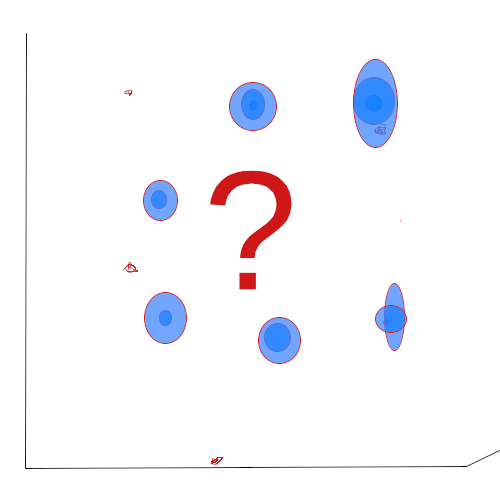
\includegraphics[scale=0.35]{images/position_plot.png}
  \caption{Positiondeviation per Coordinates in the Room}
\end{figure}

As can be seen from the figure, significant deviations were recorded outside the area enclosed by the anchors.
Even if the system is clearly capable of very precise positioning, it can be said that if uniform positioning accuracy is to be achieved,
the best arrangement of the anchors must be determined using simulation means.


\section{Conclusion And Outlook}\label{section:conclusion}
In conclusion, it can be said that a very precise localization system has been designed.
Both the hardware and the software were designed specifically for use as a positioning module and fulfill this purpose with astonishing accuracy.

A critical point is that the system is only scalable to a limited extent.
By pinging every single anchor, the tag is not able to handle a very large number of anchors without increasing the roundtrip time.
This problem could be avoided by instead of \ac{TWR} measurements \ac{TdoA} measurements would be performed.
Even if this measurement principle requires a nanosecond precise synchronization of the anchors,
the roundtrip time would be limited to the duration of one ping process.

Initially, a hybrid solution using \ac{TWR} and \ac{TdoA} measurements was sought,
but the wireless synchronization of the anchors is currently only possible with limited accuracy.
Further research in this area could allow the system to generate accurate position measurements with a period duration of up to 50ms.

To achieve further improvements, we are committed to fostering collaboration and knowledge-sharing
within the community.
Therefore, we have made the entire source code, along with all PCB design files,
readily accessible to the public.
You can find these resources, along with detailed documentation,
on our project's GitHub repository \cite{uwb-tracking}.


% Please use pisikabst.bst. You may your own *.bib file.
\bibliographystyle{pisikabst}
\bibliography{bibliography}

\end{document}